%\documentclass[12pt,letterpaper,margin=0.75in]{article}
%\documentclass[12pt]{article}

\documentclass[12pt, onecolumn]{IEEEtran}

\usepackage[utf8]{inputenc}
\usepackage{amsmath}
\usepackage{amsfonts}
\usepackage{amssymb}
\usepackage{graphicx}
\author{ECE 584 - CMOS Analog IC Design\\
SPRING 2016 - PROJECT \#1\\
}
\usepackage{geometry}

\geometry{
 letterpaper,
% total={8.5in,11in},
 left=1.0in,
 right=1.0in,
 top=1.0in,
 bottom=1.0in,
 }

\usepackage{filecontents}
\usepackage[noadjust]{cite}

\begin{filecontents*}{bibi.bib}
@ARTICLE{507173,
author={Simpson, M.L. and Young, G.R. and Jackson, R.G. and Xu, M.}, 
journal={Nuclear Science, IEEE Transactions on}, 
title={A monolithic, constant-fraction discriminator using distributed R-C delay line shaping}, 
year={1996}, 
volume={43}, 
number={3}, 
pages={1695-1699}, 
keywords={CMOS logic circuits;RC circuits;delay lines;detector circuits;discriminators;monolithic integrated circuits;nuclear electronics;20 mV to 2 V;N-well process;constant-fraction shaping;delay line;distributed R-C delay line shaping;monolithic CMOS constant-fraction discriminator;monolithic constant-fraction discriminator;slope degradation;timing errors;CMOS process;Capacitors;Circuits;Computational fluid dynamics;Delay lines;Detectors;Feedback;Laboratories;Signal generators;Timing}, 
doi={10.1109/23.507173}, 
ISSN={0018-9499}, 
month={Jun},} 
\end{filecontents*}

\title{Design and Implementation of a Nowlin Circuit}

\begin{document}

% Insert title

\maketitle

% INTRODUCTION

\section*{Introduction}

\noindent
In this first project we will start the process of designing a multi-channel discriminator chip which was described in more detail in an earlier handout. The purpose of a discriminator is to mark the arrival time of an input pulse. Ideally, the discriminator's output logic signal, marking the arrival of the input pulse, should be independent of pulse amplitude and risetime.  The discriminator in each of the 16 channels should be of the constant fraction type (CFD). In CFD discriminators an attenuated version of the input is subtracted from a delayed version of input waveform and the time at which the difference between the two signals is equal to zero is used to mark the pulse arrival time. This results in output timing signals independent of pulse amplitude. An important component of the CFD is a passive network, commonly known as a \emph{Nowlin} circuit. In this project we will design a Nowlin circuit to meet the design specification given below.

\noindent
\newline
In reality, variations in the firing time of a discriminator generally fall into two categories: time walk, $t_w$, and time jitter, $\sigma_t$. The term time "walk" is used to describe systematic variation in the rising edge of the discriminator output signal as a function of pulse height and time "jitter" describes random variation in the rising edge of the output signal due to electronic noise in the system.  We will want to design our Nowlin circuit in a manner so as to ensure excellent jitter and walk characteristics in the overall discriminator circuit.  \\  

\section*{Design Specifications}
\noindent

Your circuit must meet the following specfications.
\begin{itemize}
\item
Must support pulses of both polarities.
\item
Must accommodate signals with risetime constants ranging from 3 nsec to 100 nsec.
\item
Should exhibit excellent walk and jitter characteristics for input pulse amplitudes ranging from 20 mV to 2 V. 
\item
Must accommodate pulse repetition rates up to 1 KHz.
\item
For an input pulse with a risetime constant of 3 nsec, we require that the walk not exceed +/- 150 ps over the entire 2 mV - 2 V input amplitude range,
\item
For an input pulse with a risetime constant of 3 nsec, the jitter should not exceed 300 ps at an input level of 2 mV.
\item
The chip is to be fabricated in the ON Semiconductor, 0.5 micron CMOS process.  The targeted process supports two poly and 3 metal layers.  A high resistance poly layer is available.
\end{itemize} 
 
\section*{Overview}

\noindent
\newline
A block diagram depicting a single channel of our proposed multi-channel discriminator IC is presented in Fig.~\ref{BlockDiagram}. The Nowlin circuit is shown in detail in Fig.~\ref{Nowlin}.  The capacitor $C_0$ in the Nowlin cicuit along with the series resistance of $R_1$ and $R_2$ implement a "fast" shaper.  The output of this highpass filter is applied to the leading edge discriminator. Also, a fraction, $(\frac{R_2}{R_1 + R_2})$, of the "fast" shaper output is applied to the inverting input of the zero-cross discriminator circuit along with a delayed version of the input pulse connected to the non-inverting input. It is well-known that the time at which the differential voltage crosses through zero is independent of the input pulse amplitude.\\

\begin{figure}[htbp!]
	\centering
 	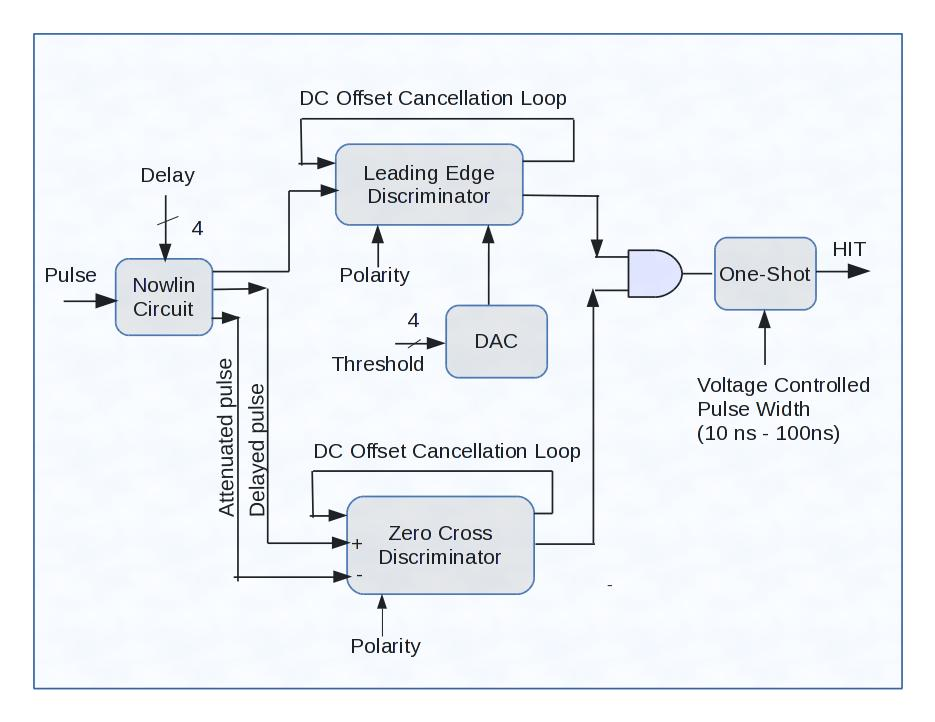
\includegraphics[scale=0.4,keepaspectratio=true]{./images/DISC16block.jpg}
 	\caption{Leading edge circuit qualifies output of zero-cross discriminator.  Leading edge and zero-cross circuits consists of a cascade of low-gain, high-bandwidth simple differential amplifiers driving a very high gain-bandwidth product (GBW) comparator }
 	\label{BlockDiagram}
\end{figure}

\begin{figure}[htbp!]
	\centering
 	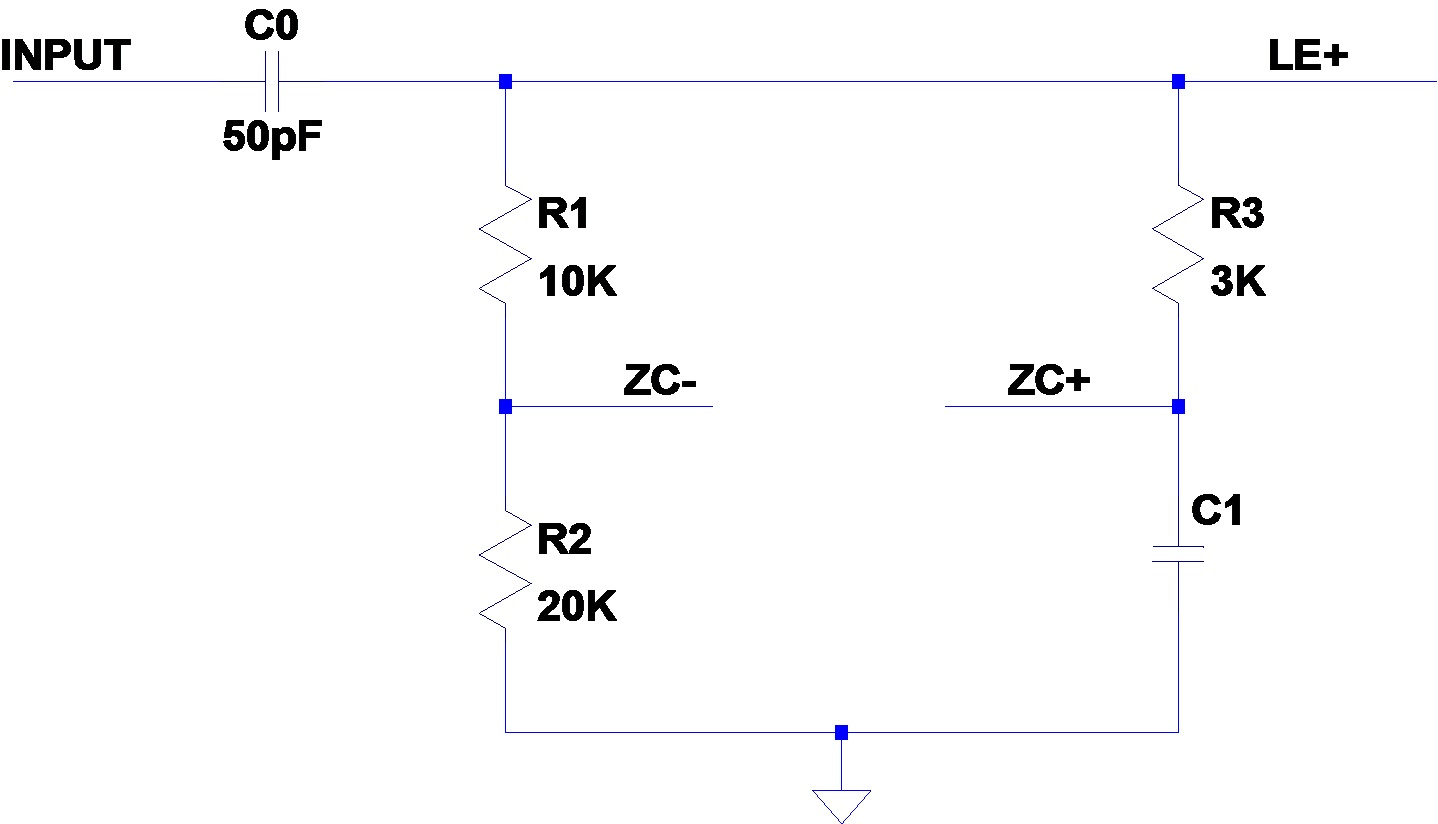
\includegraphics[scale=0.3,keepaspectratio=true]{./images/nowlin.jpg}
 	\caption{Nowlin circit using lumped components, $R_3 \text{ amd } C_1$, to implement delay. Here the fraction is $\approx$ 0.7.}
 	\label{Nowlin}
\end{figure}

\noindent
It is important that the slope (which we shall refer to as the "slew rate" or SR) of the differential signal when crossing through zero be maximized.  A delay (determined by the time constant $R_3 \cdot C_1$) which when very short will produce maximum SR but at the expense of underdrive voltage. In Fig.~\ref{TypicalWaveforms} the input pulse risetime constant is 3 ns (in other words,  a 10 - 90 \% rise time of 6.6 ns).  When the time constant in the Nowlin circuit is 300 ps, the SR is high but the underdrive is quite small. The underdrive must be sufficiently large so as to drive the comparator output to the logic false state.  Remember, that Fig.~\ref{TypicalWaveforms} remains essentially unchanged when the peak pulse amplitude is reduced to 20 mV except all amplitudes are 1 \% of the values shown in the figure. When the time constant in the Nowlin circuit is 6 ns, the underdrive voltage is high but the SR suffers. Clearly, when the time constant is 1.5 ns, a good compromise between SR and underdrive voltage is achieved. In the proposed design, capacitor $C_1$ and/or resistor $R_3$ will be programmable. In this way, the delay can be matched to the risetime of the input pulse and we can accommodate a wide range of input rise time constants. \\

\begin{figure}[htbp!]
	\centering
 	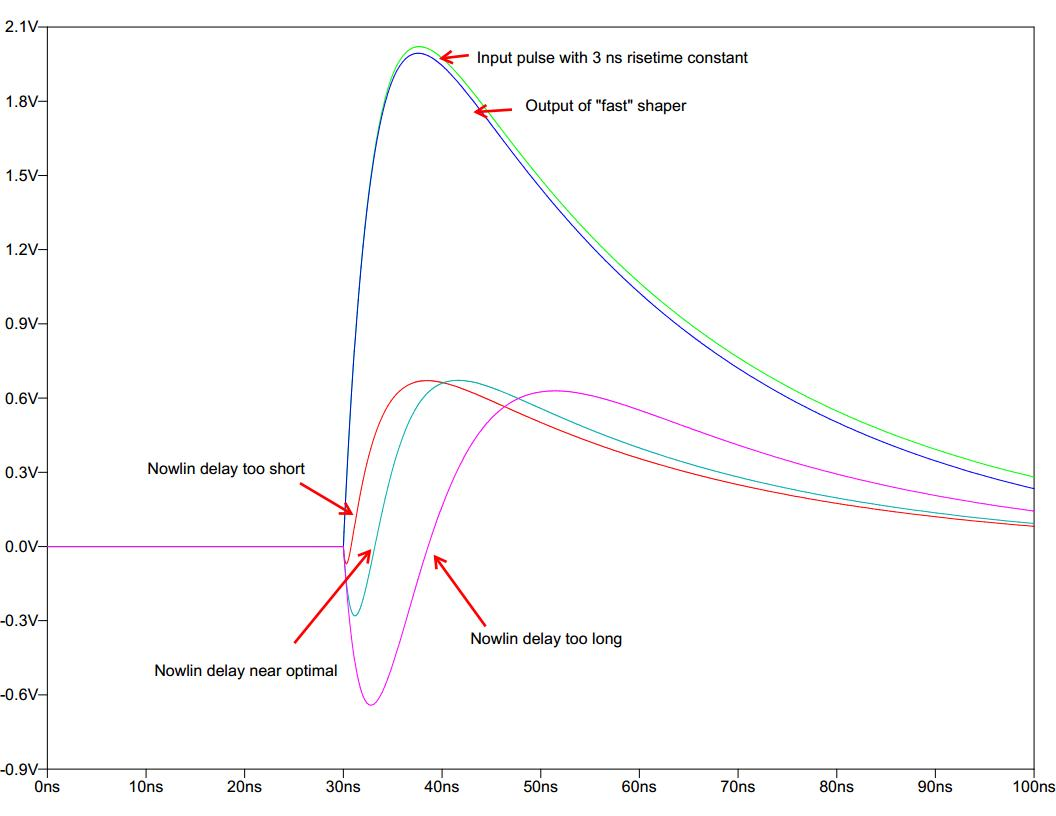
\includegraphics[scale=0.4,keepaspectratio=true]{./images/nowlin_fast.jpg}
 	\caption{Input signal with 3 ns risetime constant. A programmable delay allows matching of the delay provided by the Nowlin circuit to the risetime constant of the input signal.}
 	\label{TypicalWaveforms}
\end{figure}

\section*{Deliverables}

\noindent


\end{document}